%
%	Begrifflichkeiten
%

\pagebreak
\section{Data definition and wrangling}

\onehalfspacing

\subsection{Data Source}

\subsubsection{The Group}

Bla bla

\subsubsection{The Blog}

At the following URL: \url{https://koelle4future.de/}

Bla bla

In this paper, I will look at my blog's traffic data, analyze that data, and then lay the foundation to predict a blog post's performance based on its content.

\subsubsection{Social Media and Loneliness}

In the current COVID-19 pandemic, social distancing is a key element in containing the virus's spread. Social distancing over a long period of time can increase loneliness and significantly affect people's health negatively, according to a recent study conducted by the American Psychological Association.\footnote{See \textit{Luchetti, M. (2020)}: The trajectory of loneliness in response to COVID-19. \cite{apaLoneliness}}

In the study, the researchers formulate the hypothesis that an increase in perceived support from others can offset loneliness during the required isolation.

One element to offset the effects of loneliness is increased interaction on social media and virtual meetings with video. Social media interaction includes reading blogs - the more engaging a blog post is, the more chances it has to reach people to whom it will be entertaining or otherwise beneficial.

Thus this analysis aims to get an answer for my blog on the question "On which subject(s) should I post to increase my reach?". We will be using visualization and correlation as the primary means of analysis to increase the value of the blog for others.

\subsubsection{Covid-19 and Hate Speech}

Violence in Language\footnote{See \textit{Brown, L.X.Z. (2014)}: Violence in Language. \cite{violenceLanguage}}

Bla bla\footnote{See \textit{UNAIDS (2020)}: Addressing stigma and discrimination. \cite{addressingStigma}}

Bla bla\footnote{See \textit{TIME's UP (2020)}: Equity and Inclusion During Crisis. \cite{equityInclusion}}

Good example: "Covidio***"\footnote{See \textit{Juterczenka, J.v. (2021)}: Begriff "Covidio***". \cite{covidioXXX}}

A handy reference to the terms\footnote{\textit{Brown, L.X.Z. (2021)}: Ableism/Labguage. \cite{ableismLanguage}}

\subsubsection{Climate Anxiety}

Bla bla\footnote{See \textit{Dellinger, AJ. (2021)}: The connection between climate anxiety and white fragility. \cite{climateAnxiety}}

\subsection{Web Traffic Analysis}

Web analytics is the domain of the big search engines, and Google Analytics and Google AdSense are the market leaders, followed by Microsoft Bing Web Analytics. In all of Social Media and Social Media Marketing, web analytics plays a crucial role in evaluating a website's performance and forms the basis of automated advertising placement.

Advertising, as much as we might dislike it, pays for most of the content we consume.

Page views, bounce rate, and unique visitors are key metrics to evaluate a website and the currency that fuels the internet. Every marketeer or web site owner will use these metrics to analyze performance and identify areas for growth; many tools for analysis have become available in the last couple of years, some of them open-source, some closed-source.

Generally speaking, more traffic can potentially lead to more business opportunities. It is mandatory for a commercial website to monitor its web analytics data daily and act immediately on any anomaly.

However, a blog does not necessarily have commercial interests and might be an outlet for personal interests or interactions. Why would we want to look at web analytics anyway?

\subsection{Web Traffic KPIs}

In marketing categories, a blog belongs to inbound marketing, as it tries to offer engaging content and create value for the visitors but does not reach out by itself. 

Unlike outbound email campaigns, for example, that ask the visitor to view a particular website, a blog relies on its content and the willingness of the visitor to actively choose the site for a visit, for example, by being pointed to a post from a Google search result or a tweet.

In WordPress, there is an option to subscribe to a blog to get a notification on new posts; WordPress also provides the ability to subscribe to a blog's RSS feed. Even though, as this requires active user interaction and interest, blogs are considered an inbound channel.

In a recent paper on inbound marketing, Yvonne Romes identifies a couple of important KPIs for inbound marketing, a couple of which I will summarize here based on her paper:\footnote{See \textit{Romes, Y. (2020)}: 10 Inbound KPIs, die jetzt auch Personaler kennen sollten. \cite{inboundKPI}}

\begin{itemize}
\item Page Views
\item Bounce Rate
\item Visit Duration
\item Unique Visitors
\end{itemize}

Page Views is the number of clicks a specific page has received; on a blog, more page views indicate more engaging content.

Bounce Rate describes the rate of users that leave the site without selecting another link; a high bounce rate can indicate a lack of engaging or interesting content.

Visit Duration is the amount of time a unique visitor spends on the website; for a blog that mainly offers content to read, a longer duration most likely indicates higher engagement.

A unique visitor is a visitor that can be differentiated from another visitor. Unlike many other platforms, Plausible does not use tracking cookies to identify individual visitors but relies on publicly available information, such as an IP address, to differentiate them. Even though the metric is less accurate with Plausible than with other platforms, it's still an important metric, and as before, on a blog, more visitors usually indicate higher engagement.

In this paper, these are the four metrics that I will focus on.

\subsection{Data Collection}

Data exported from the Kölle for Future Blog wp-statistics module as CSV files\footnote{See \textit{VeronaLabs OÜ (2021)}: Documentation. \cite{wpStatistics}}

\subsection{Data Wrangling}

\subsubsection{Original Columns}

Let's have a look at the original columns

\begin{lstlisting}[caption=wp-admin, frame=single, basicstyle=\ttfamily]
"date", "IP", "hostname"
\end{lstlisting}

\begin{lstlisting}[caption=wp-comments, frame=single, basicstyle=\ttfamily]
"comment-ID", "comment-post-ID", "comment-author", 
"comment-author-email", "comment-author-url", 
"comment-author-IP", "comment-date", "comment-date-gmt", 
"comment-content", "comment-approved", "comment-parent", 
"comment-type", "user-id", "comment-alter-id", 
"meta:ct-checked", "meta:ct-checked-now", "meta:ct-bad", 
"meta:ct-hash", "meta:akismet-result", 
"meta:akismet-history", "meta:akismet-as-submitted"
\end{lstlisting}

\begin{lstlisting}[caption=wp-pages, frame=single, basicstyle=\ttfamily]
"page-id", "uri", "type", "date", "count","id"
\end{lstlisting}

\begin{lstlisting}[caption=wp-search, frame=single, basicstyle=\ttfamily]
"ID", "last-counter", "engine", "host", "words", "visitor"
\end{lstlisting}

\begin{lstlisting}[caption=wp-visit, frame=single, basicstyle=\ttfamily]
"ID", "last-visit", "last-counter", "visit"
\end{lstlisting}

\begin{lstlisting}[caption=wp-visitor, frame=single, basicstyle=\ttfamily]
"ID", "last-counter", "referred", "agent", 
"platform", "version", "UAString", "IP", 
"location", "user-id", "hits", "honeypot"
\end{lstlisting}

\subsubsection{Removing PII}

\begin{itemize}
 \item wp-admin: Just affecting the author, no change necessary
 \item wp-comments: We're removing anything that could identify the commenter as well as all meta information and ab empty column.
 \item wp-pages: No personally identifiable information
 \item wp-search: No personally identifiable information
 \item wp-visit: No personally identifiable information
 \item wp-visitor: We'll remove all admin access and are removing anything that could identify the visitor
\end{itemize}

\subsubsection{GDPR}

We can assume that wp-statistics is not GDP-compliant from the amount of data that we need to remove, even though it claims that it is (see Matomo blog\footnote{See \textit{Kohr, J. (2020)}: Matomo vs WP-Statistics. \cite{matomoBlog}}). Furthermore, there is no information visible on the blog that we will process data, as required by DS-GVO. The collection of IP addresses is difficult to justify. Lessons learned:

\begin{itemize}
 \item Enable Geo-IP location data
 \item Disable collection of IP addresses
\end{itemize}

\subsubsection{Removing Spam}

\begin{lstlisting}[caption=Shell script: Removing Spam, frame=single, basicstyle=\ttfamily]
$ wc -l wp-visitor-2021-04-05.csv
68027 wp-visitor-2021-04-05.csv

$ fgrep -e "DE" wp-visitor-2021-04-05.csv | wc -l
49883

$ fgrep -e "AT" wp-visitor-2021-04-05.csv | wc -l
519

$ fgrep -e "CH" wp-visitor-2021-04-05.csv | wc -l
264

$ fgrep -e "CH" -e "AT" -e "DE" wp-visitor-2021-04-05.csv \
  > wp-visitor-2021-04-05-nospam.csv

$ wc -l wp-visitor-2021-04-05-nospam.csv 
50564 wp-visitor-2021-04-05-nospam.csv
\end{lstlisting}

\subsection{Count}

To analyze and visualize the data, I'll be using data notebooks from Count. Like Jupyter notebooks that combine (Python) Code and Text, the data notebooks combine (SQL) Data and Text in a pretty ingenious way. Data notebooks support data-driven decision making, and have recently come out of open beta.\footnote{See \textit{Count.co (2020)}: About Count. \cite{aboutCount}}

\subsubsection{Database}

Creating a BiqQuery database on Google Cloud and connecting a Count data notebook with a read-only service account

\begin{figure}[H]
\centering
\caption {Database Tables}
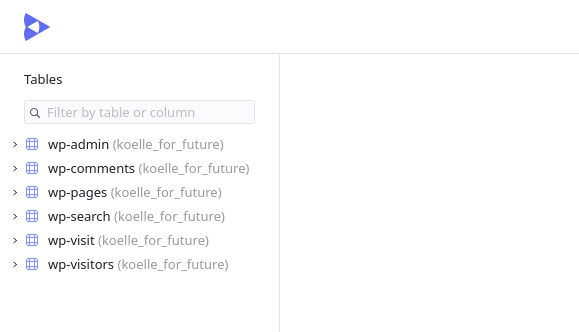
\includegraphics[width=\linewidth]{images/tables.png}
\label{fig:tablesCount}
\end{figure}
